\section{Define Logical Architecture}
\label{section:define-logical-architecture}

Nine logical components realize F01--F08 without specifying implementation technologies \citep[Sec.~17.3.4]{friedenthal2014practical}. Learning, finances, RAM, credibility, software and technician concerns extend the response beyond evidence custody. El Hachimi et al. inform mission-driven sizing, component and thermal/EMC decisions, protection and telemetry checks \citep[Secs.~2--5 and~8.1.6--8.1.7]{handpicked-0003}. The Handbook informs coordinated requirements, budgets, interfaces and verification planning \citep[Secs.~I.3--I.4]{aguado2021cubesatse}. Their EPS results remain case-specific.

\subsection{Responsibilities and allocations}

Figure~\ref{fig:framework-logical} presents three views of the same nine logical components, with their important records, required information and provided services. Each dashed reference refers to an existing component, not an additional component or deployment. FR numbers identify the 40 primary responsibility allocations. Supporting responsibilities and exchanges remain formalized in the SysML v2 model. This decomposition imposes no executable or node count. Intended allocation is not demonstrated requirements satisfaction \citep[Sec.~17.3.7]{friedenthal2014practical}.

% One figure, continued across three pages to keep the native summaries readable.
\begin{figure}[p]
\centering
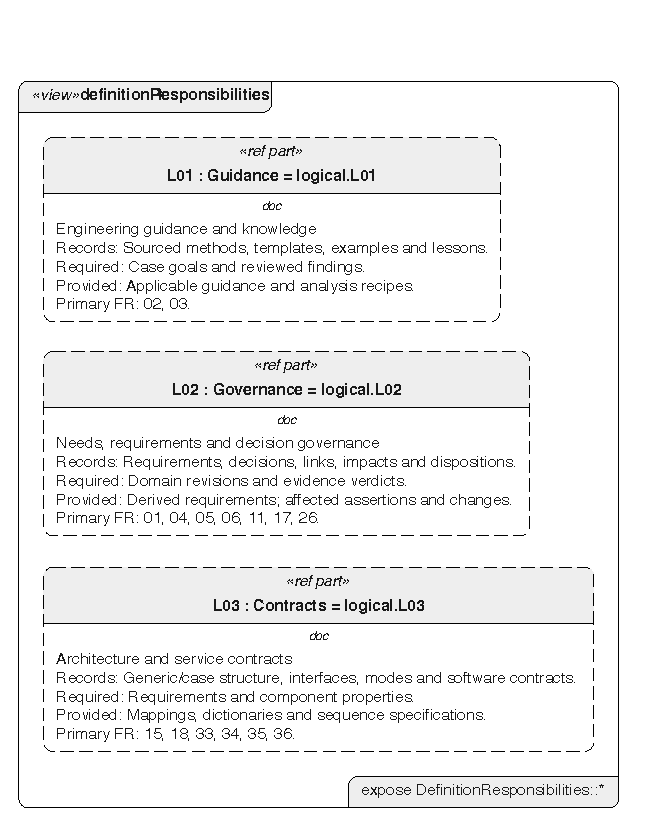
\includegraphics[width=\linewidth,height=0.84\textheight,keepaspectratio]{fig/sysml/logical/sysml-defined-view-logicalresponsibilityviews-definitionresponsibilities.pdf}
\caption{Logical component responsibilities, records and required/provided services. Primary FR numbers state intended allocation, not demonstrated satisfaction. (a) L01--L03: guidance, governance and architecture.}
\label{fig:framework-logical}
\end{figure}
\begin{figure}[p]
\ContinuedFloat
\centering
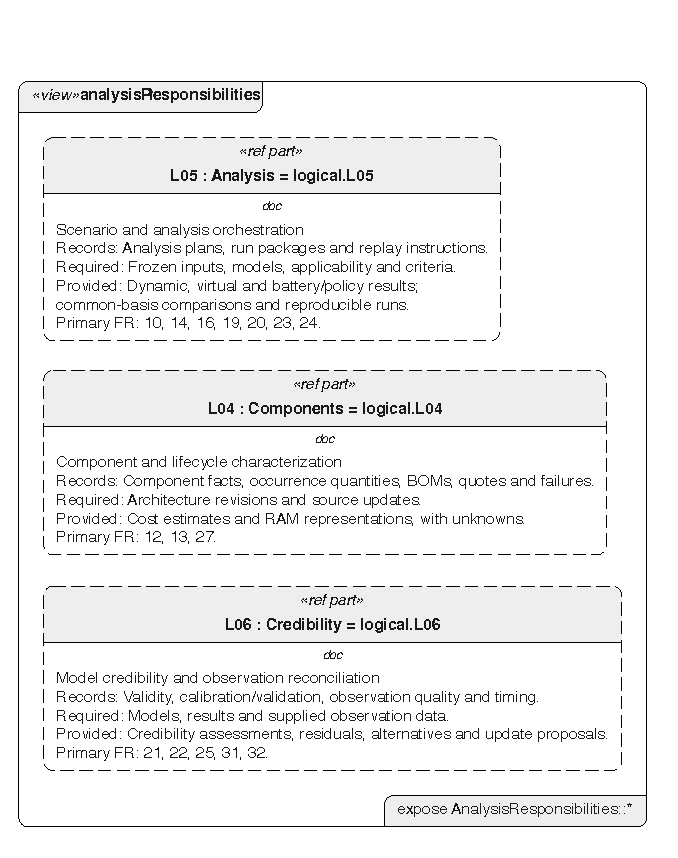
\includegraphics[width=\linewidth,height=0.84\textheight,keepaspectratio]{fig/sysml/logical/sysml-defined-view-logicalresponsibilityviews-analysisresponsibilities.pdf}
\caption[]{Logical component responsibilities (continued). (b) L04--L06: characterization, analysis and credibility.}
\end{figure}
\begin{figure}[p]
\ContinuedFloat
\centering
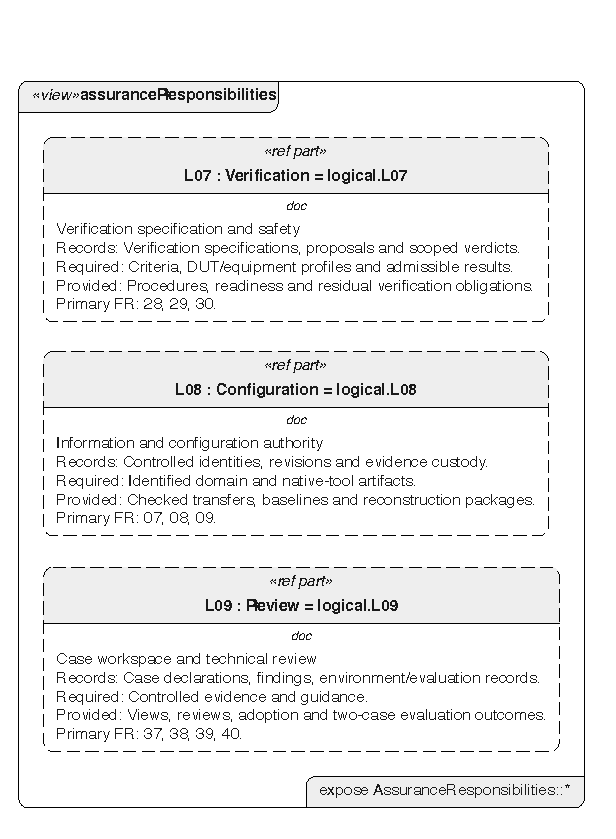
\includegraphics[width=\linewidth,height=0.84\textheight,keepaspectratio]{fig/sysml/logical/sysml-defined-view-logicalresponsibilityviews-assuranceresponsibilities.pdf}
\caption[]{Logical component responsibilities (continued). (c) L07--L09: verification, configuration and review.}
\end{figure}
\clearpage

\subsection{Typed exchanges, authority and feedback}
{\small
\setlength{\tabcolsep}{4pt}
\setlength{\parskip}{0pt}
\setlength{\LTpre}{0.4\baselineskip}
\setlength{\LTpost}{0.4\baselineskip}
\renewcommand{\arraystretch}{1.06}
\begin{longtable}{@{}>{\raggedright\arraybackslash}p{\dimexpr0.32\linewidth-0.64\tabcolsep\relax}>{\raggedright\arraybackslash}p{\dimexpr0.68\linewidth-1.36\tabcolsep\relax}@{}}
\caption{Information exchanges between logical components.}\label{tab:framework-logical-exchanges}\\
\toprule
\textbf{Participants} & \textbf{Exchanged information and required handling} \\
\midrule
\endfirsthead
\caption[]{Information exchanges between logical components. (continued).}\\
\toprule
\textbf{Participants} & \textbf{Exchanged information and required handling} \\
\midrule
\endhead
\bottomrule
\endfoot
All $\leftrightarrow$ L08 & Registration, transfer verdict, exact manifest and reconstruction. Check envelope/semantics/provenance and preserve rejected/prior revisions. \\
L02 $\leftrightarrow$ L03/L04/L06/L07 & Requirements, criteria, impact and domain revision proposals. Resolve dependencies and retain stale/unresolved evidence. \\
L03/L04/L06/L07 $\rightarrow$ L05 & Occurrences, characterization, failure dependencies, applicable models and verification criteria freeze the run. Software mappings also drive sequence/resource checks. \\
L05 $\rightarrow$ L06 $\rightarrow$ L07 $\rightarrow$ L02 & Raw analysis results, model credibility assessment, verification verdict based on admissible evidence and status of affected technical assertions. Supplied observations return through proposed parameter/design updates. \\
L01/L09 $\leftrightarrow$ domain owners & Guidance, baseline-linked reviews, findings and lessons. Apply tailoring, return findings to owners and separate local learning from general source claims. \\
\end{longtable}
}

L08 controls accepted baselines and consistent identification. Each domain component remains responsible for the meaning of its information: requirements (L02), architecture and interfaces (L03), component characteristics (L04), models and observations (L06), verification (L07), knowledge (L01) and case reviews (L09). Generated analysis inputs, software definitions and views refer to these controlled sources rather than creating competing definitions. Mission software behavior and deployment still require separate implementation and verification \citep[Secs.~3--5]{review-0853}.

Interface specifications for quantities, signs, reference frames, clocks and validity address model, degradation, sensor and timing effects \citep[Secs.~4.1--4.2 and~6]{review-1251}. Numerical step size proves no real-time suitability \citep[Sec.~3]{review-0573}. SC01 follows guidance and definition, analysis, credibility assessment, verification and review. SC02 evaluates change impacts through domain revisions and reanalysis. SC03 uses failed checks or supplied observations to propose updates and safe verification activities. Design change, observation reconciliation and reviewed learning share L08 revision control. They never silently overwrite earlier evidence or actuate hardware.
